\section{DNS Security}

The Internet is a critical infrastructure, yet its operation depends on the fundamentally insecure DNS. DNS provides a mapping of names to resources of several types. However, DNS, as a robust key protocol of the Internet, is also a formidable attack vector for cyber criminals:

\begin{itemize}
	\item Manipulating the DNS mapping allows an attacker to redirect connections to malicious server, facilitate MitM attacks and launch DoS attacks.
	\item DNS helps building hidden channels (tunneling)
	\item is abused for powerful denial of service attacks
	\item is abused for various impersonation attacks
	\item used to setup services that are hard to hunt-down or shut-down (Botnets, Fast- & Domain Flux)
\end{itemize}

\subsection{Domain Name System (DNS)}
DNS is a globally distributed, loosely coupled, scalable, reliable and dynamic database. DNS data is maintained locally and retrievable globally, no single computer has all DNS data. 
DNS uses hierarchical namespaces to scale: tree structure down from root level ".", to top-level domains (TLD, e.g. .com) to second-level domains (SLD, e.g. google.com). A fully qualified domain name (FQDN) for example is mail.ethz.ch. The hierarchy descends from right to left. Domains are namespaces: everything below .com is the \textit{com} domain, everything below .ibm.com. is the \textit{ibm.com} domain.

\begin{minipage}{\linewidth}
    \centering      
    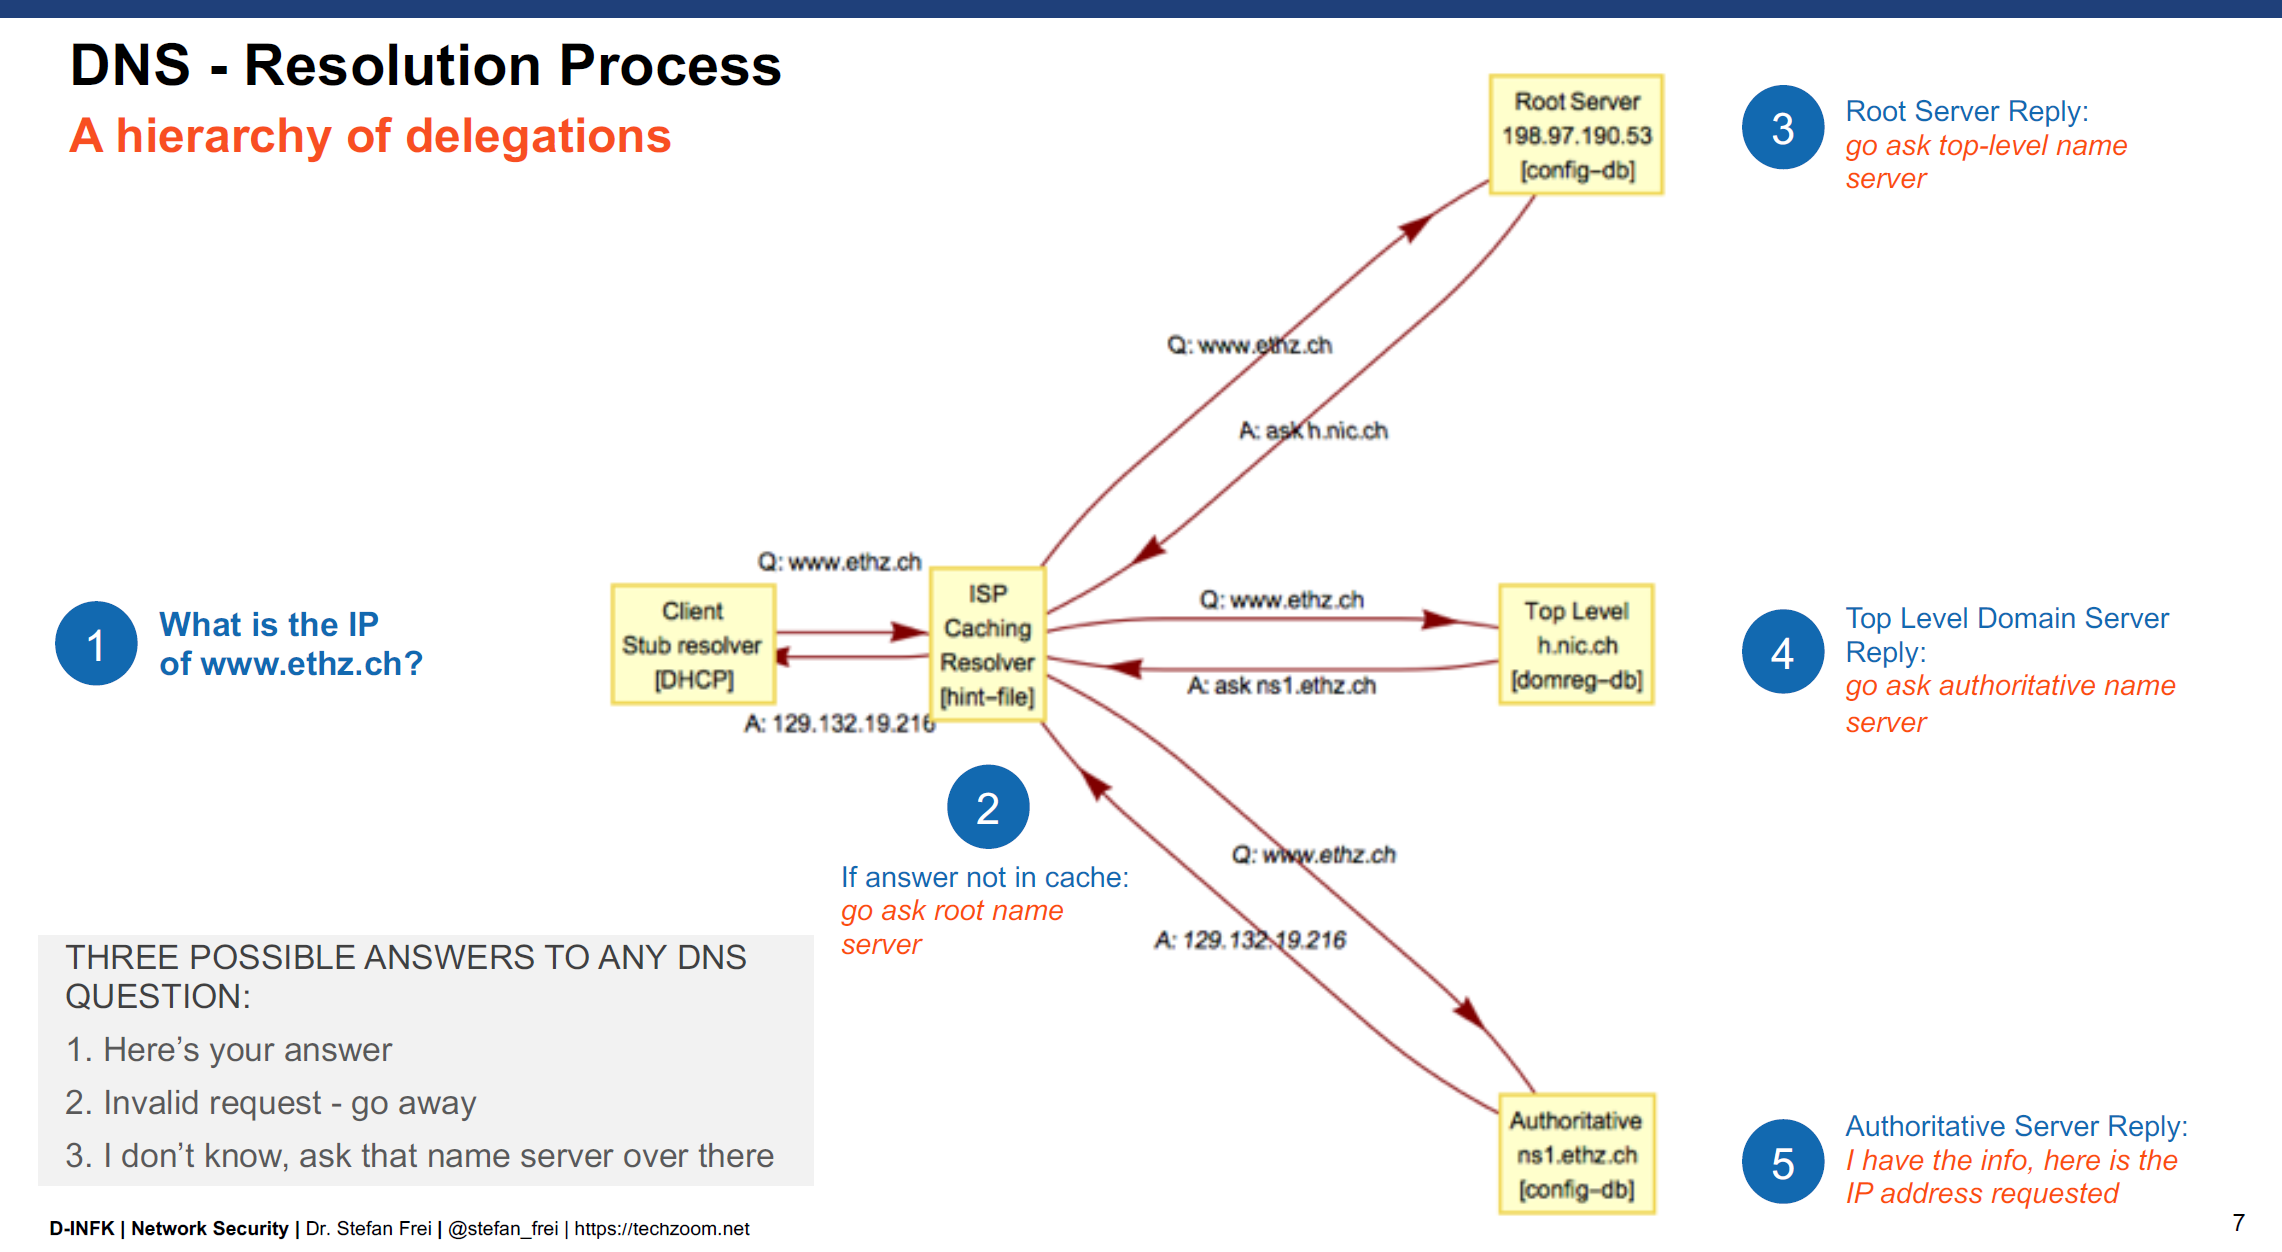
\includegraphics[width=\linewidth]{Figures/DNS_resolution.PNG} 
\end{minipage}

\subsection{DNS Protocol Features}
The DNS protocol was designed with a mechanism to protect against forged responses. The first two bytes in the message form a transaction ID (txid) that must be the same in the query and response.

\begin{itemize}
	\item Protocol: simple client-server protocol, operating on TCP/UDP port 53. No encryption, authentication nor integrity built into original protocol.
	\item Name server: Servers that map names to objects (= resource records RR). Authoritative: server is authoritative for a specific zone. Caching/Resolver: server resolves domains recursively, caches results.
	\item Client sends query and random txid, dnsserver responds with query, txid, response.
	\item Resolver: Client side of DNS resolution, responsible for initiating and sequencing the queries that ultimately lead to a full resolution. Stub resolver: piece of software running on a client that sends recursive DNS requests to a recursive resolver. Recursive resolver: processes DNS resolution iteratively to	provide full answer: it contacts all the different servers at the different domain levels to get the final answer.
\end{itemize}

\begin{minipage}{\linewidth}
    \centering      
    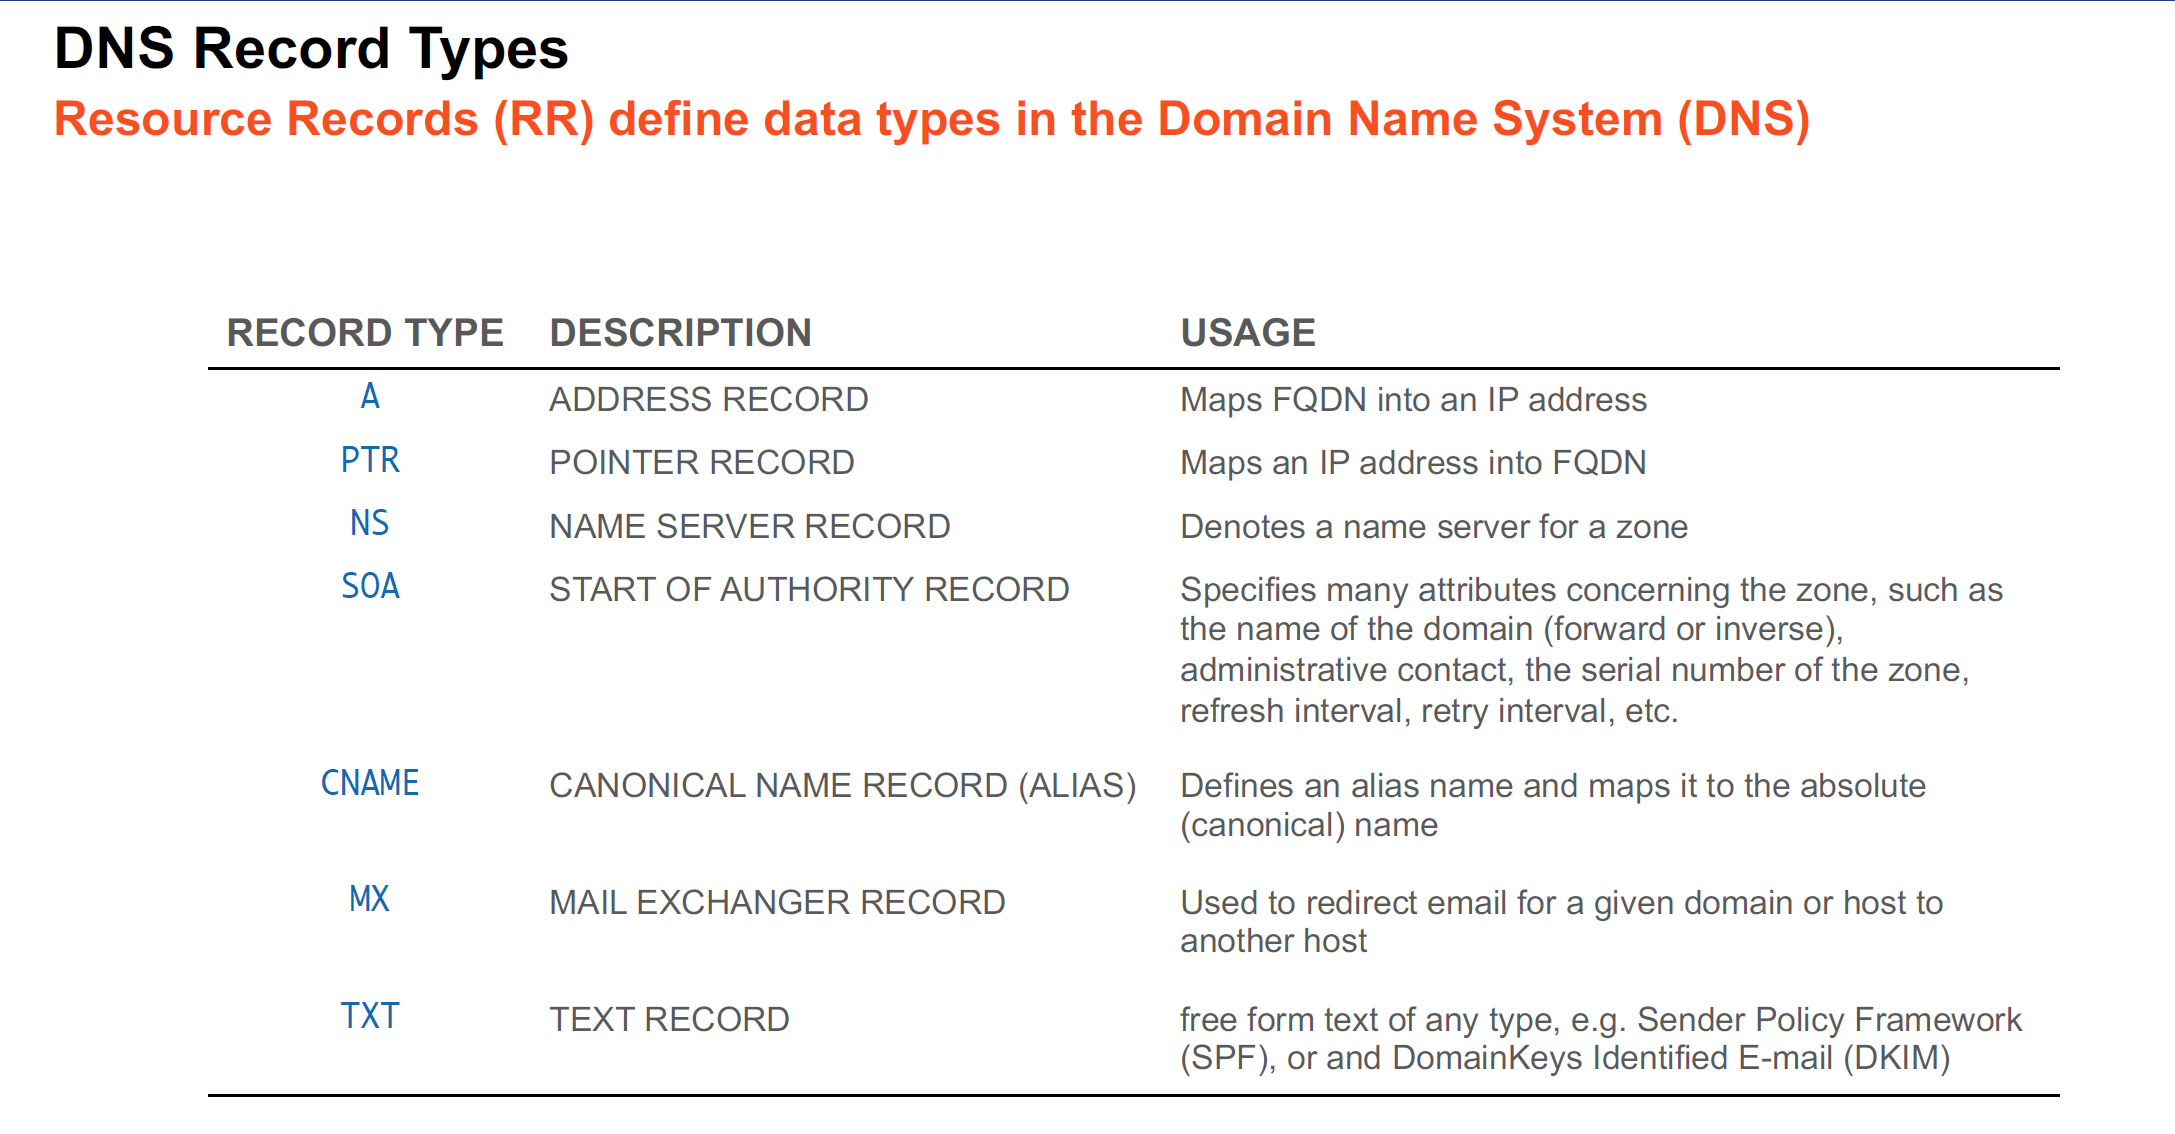
\includegraphics[width=\linewidth]{Figures/DNS_record_types.PNG} 
\end{minipage}

\paragraph{DNS Caching:}
We want to decrease lookup latency and network traffic. Each DNS response has a TTL. Caching resolvers will redo a recursive lookup once the TTL for a cached response has expired. A shorter TTL leads to shorter living cache entries, leading to faster refreshes for end users in case of an update. However, this means that there will be more load on the DNS servers for doing the recursive lookup again.

\paragraph{Attack Patterns:}
Insert tampered information into DNS server or resolution process. Control DNS of all clients served by name server/resolver

\begin{minipage}{\linewidth}
    \centering      
    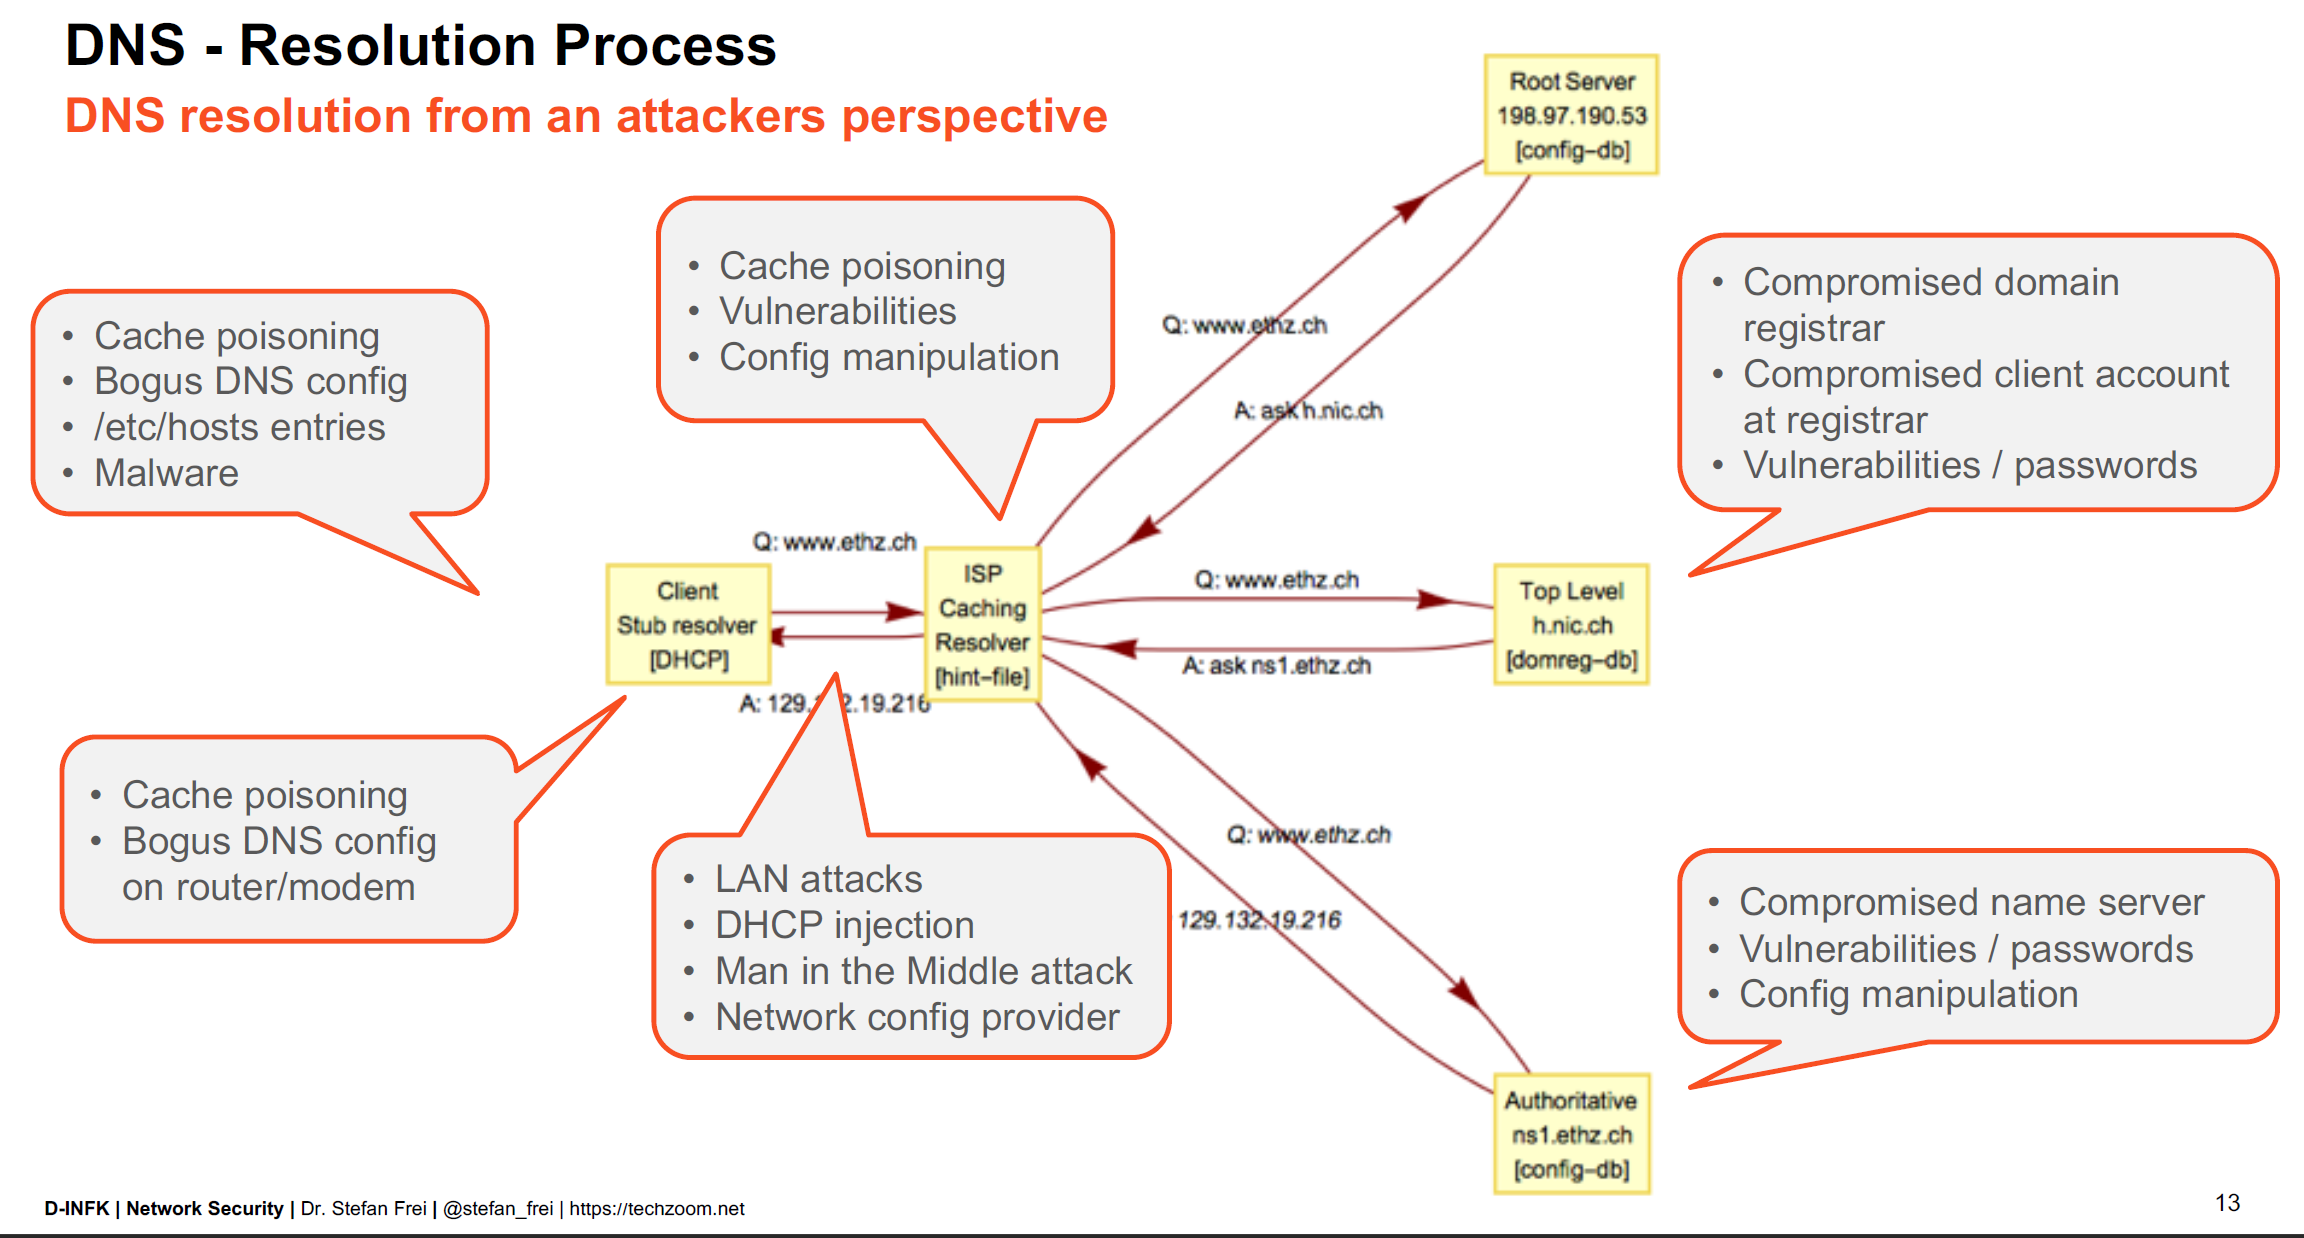
\includegraphics[width=\linewidth]{Figures/DNS_attacker_perspective.PNG} 
\end{minipage}

\begin{minipage}{\linewidth}
    \centering      
    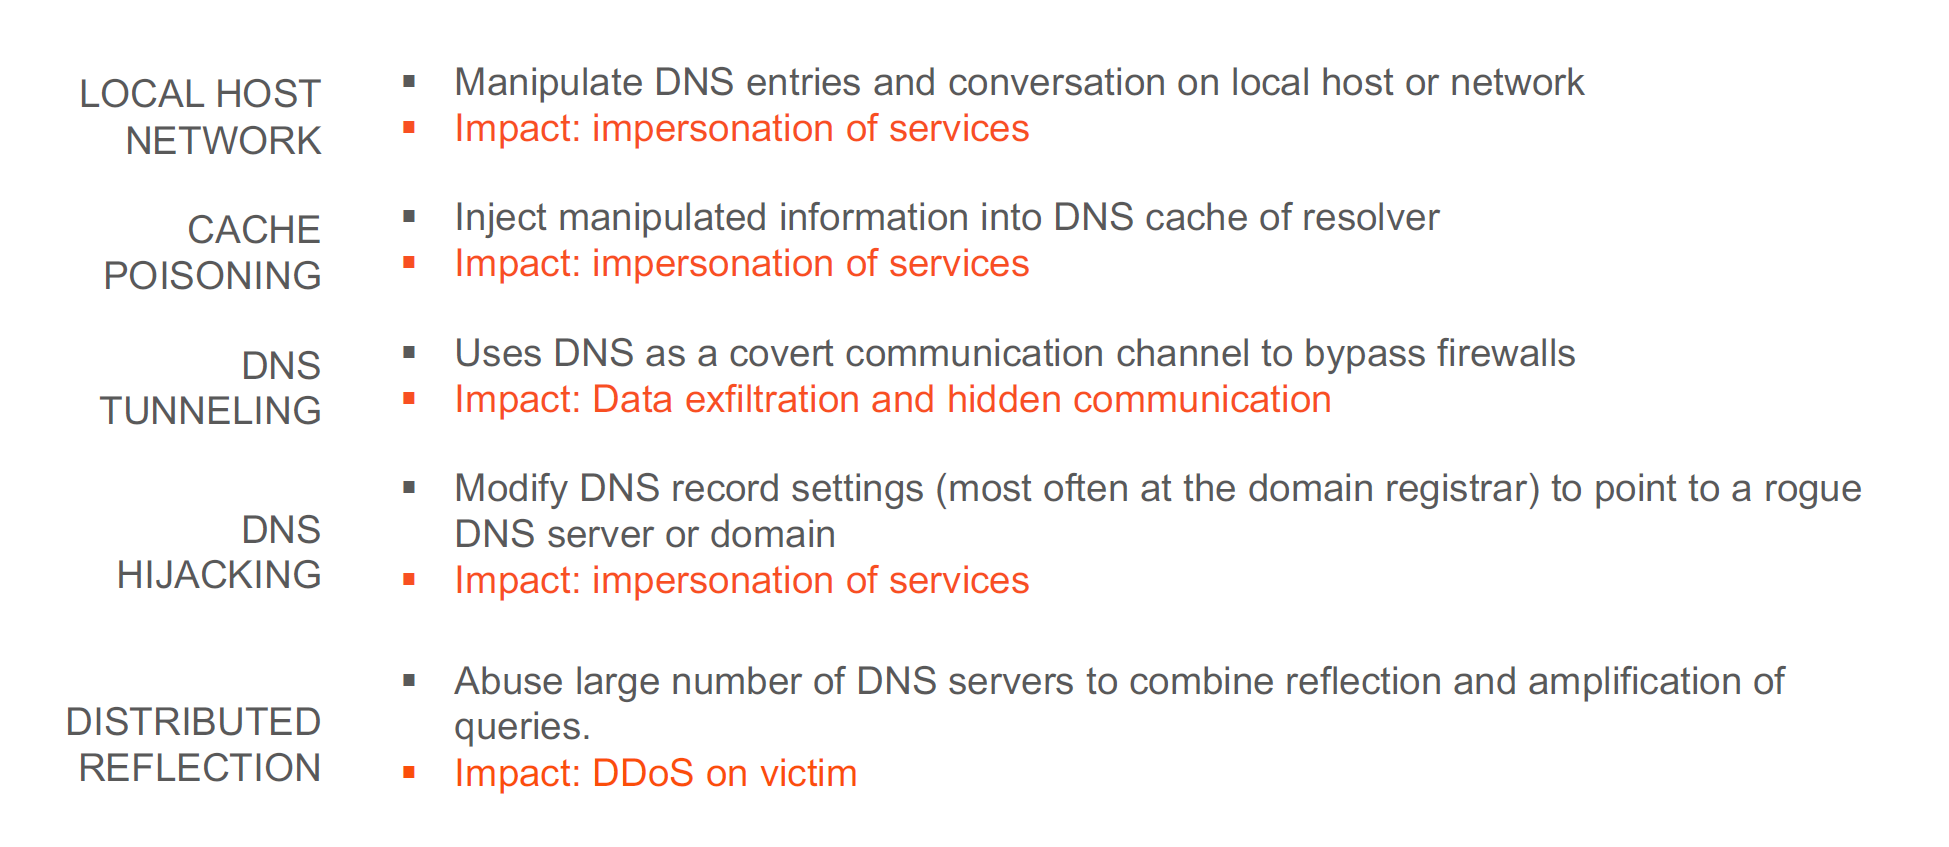
\includegraphics[width=\linewidth]{Figures/DNS_common_attacks.PNG} 
\end{minipage}

\subsubsection{Root servers}

\paragraph{DNS Root Zone:}
DNS root name servers are the key to the Internet kingdom: the DNS root zone is served by 13 root server clusters which are authoritative for queries for the top level domains. Every name resolution in the Internet either starts with a query to a root server, or, uses information that was once obtained from a root server. DNS root name servers have the official names a.root-servers.net to m.root-servers.net. They only resolve the IP addresses for the top-level name servers (TLD). The bandwidth available at RSS (Root Server System) is significant but no immune to DoS. Try to vary hardware in RSS to limit effects of a vulnerability.

\paragraph{Top-Level name servers}
A domain name registrar is an organization that manages the reservation of second-level Internet domain names (SLD) below a given top-level domain (TLD). A domain name registrar must be accredited by a top-level domain registry and/or a country code top-level domain (ccTLD) registry. Based on the domain registration database, the top-level name server points resolvers to the authoritative name server of the SLD.

\paragraph{Authoritative Domain Server}
The authoritative name server for a second-level domain is managed by private entities or on behalf of private entities that have registered a domain name. The authoritative name server has all records for a zone configured and can provide the final / authoritative information.

\subsection{Cache Poisoning}
\begin{minipage}{\linewidth}
    \centering      
    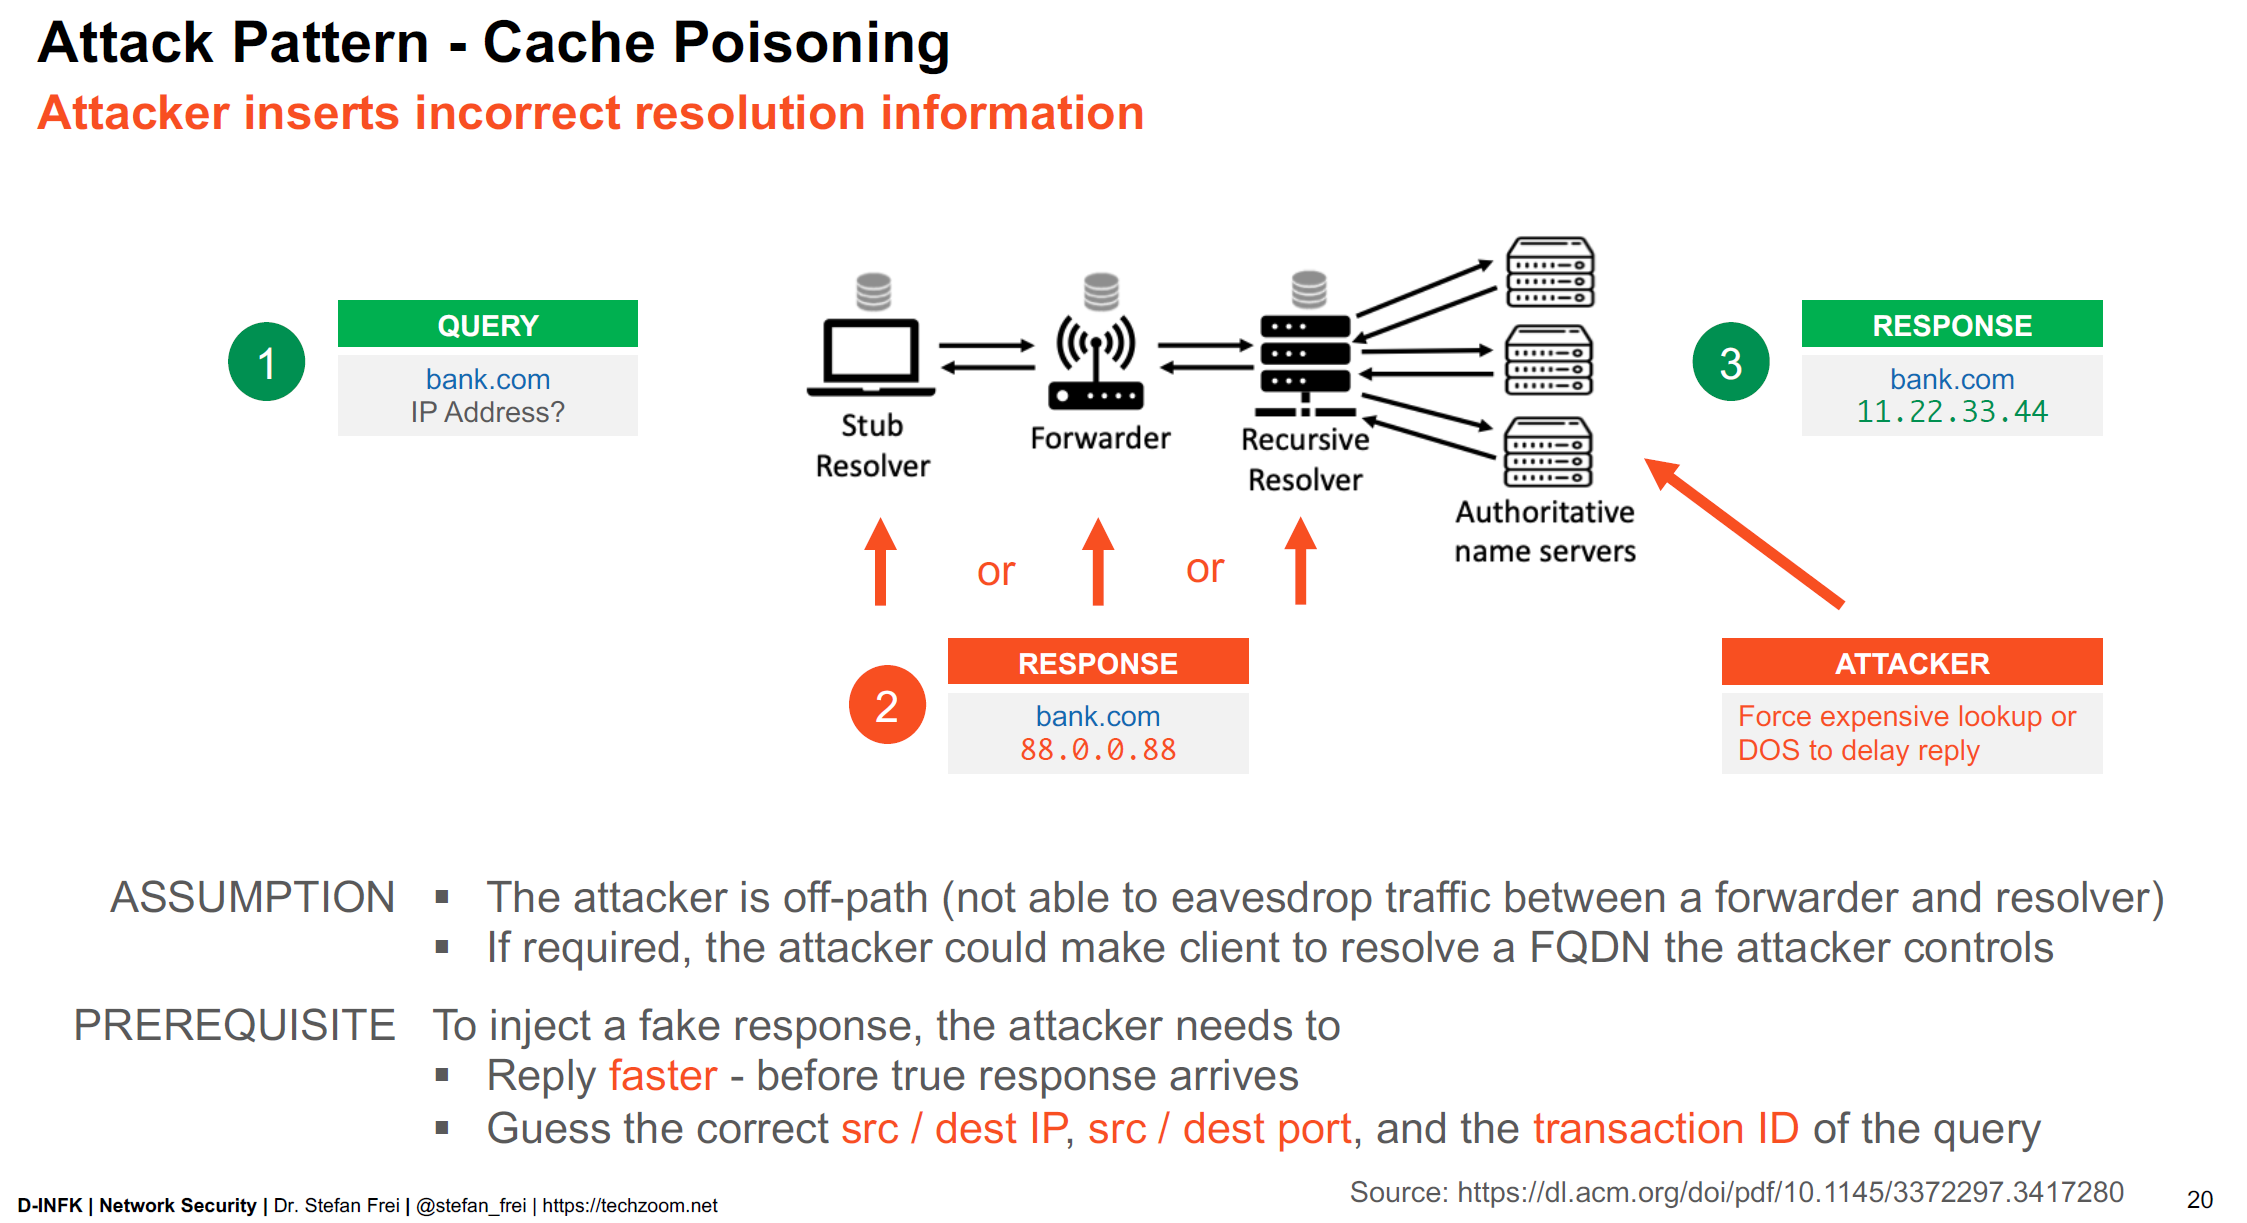
\includegraphics[width=\linewidth]{Figures/DNS_cache_poisoning.PNG} 
\end{minipage}

\begin{minipage}{\linewidth}
    \centering      
    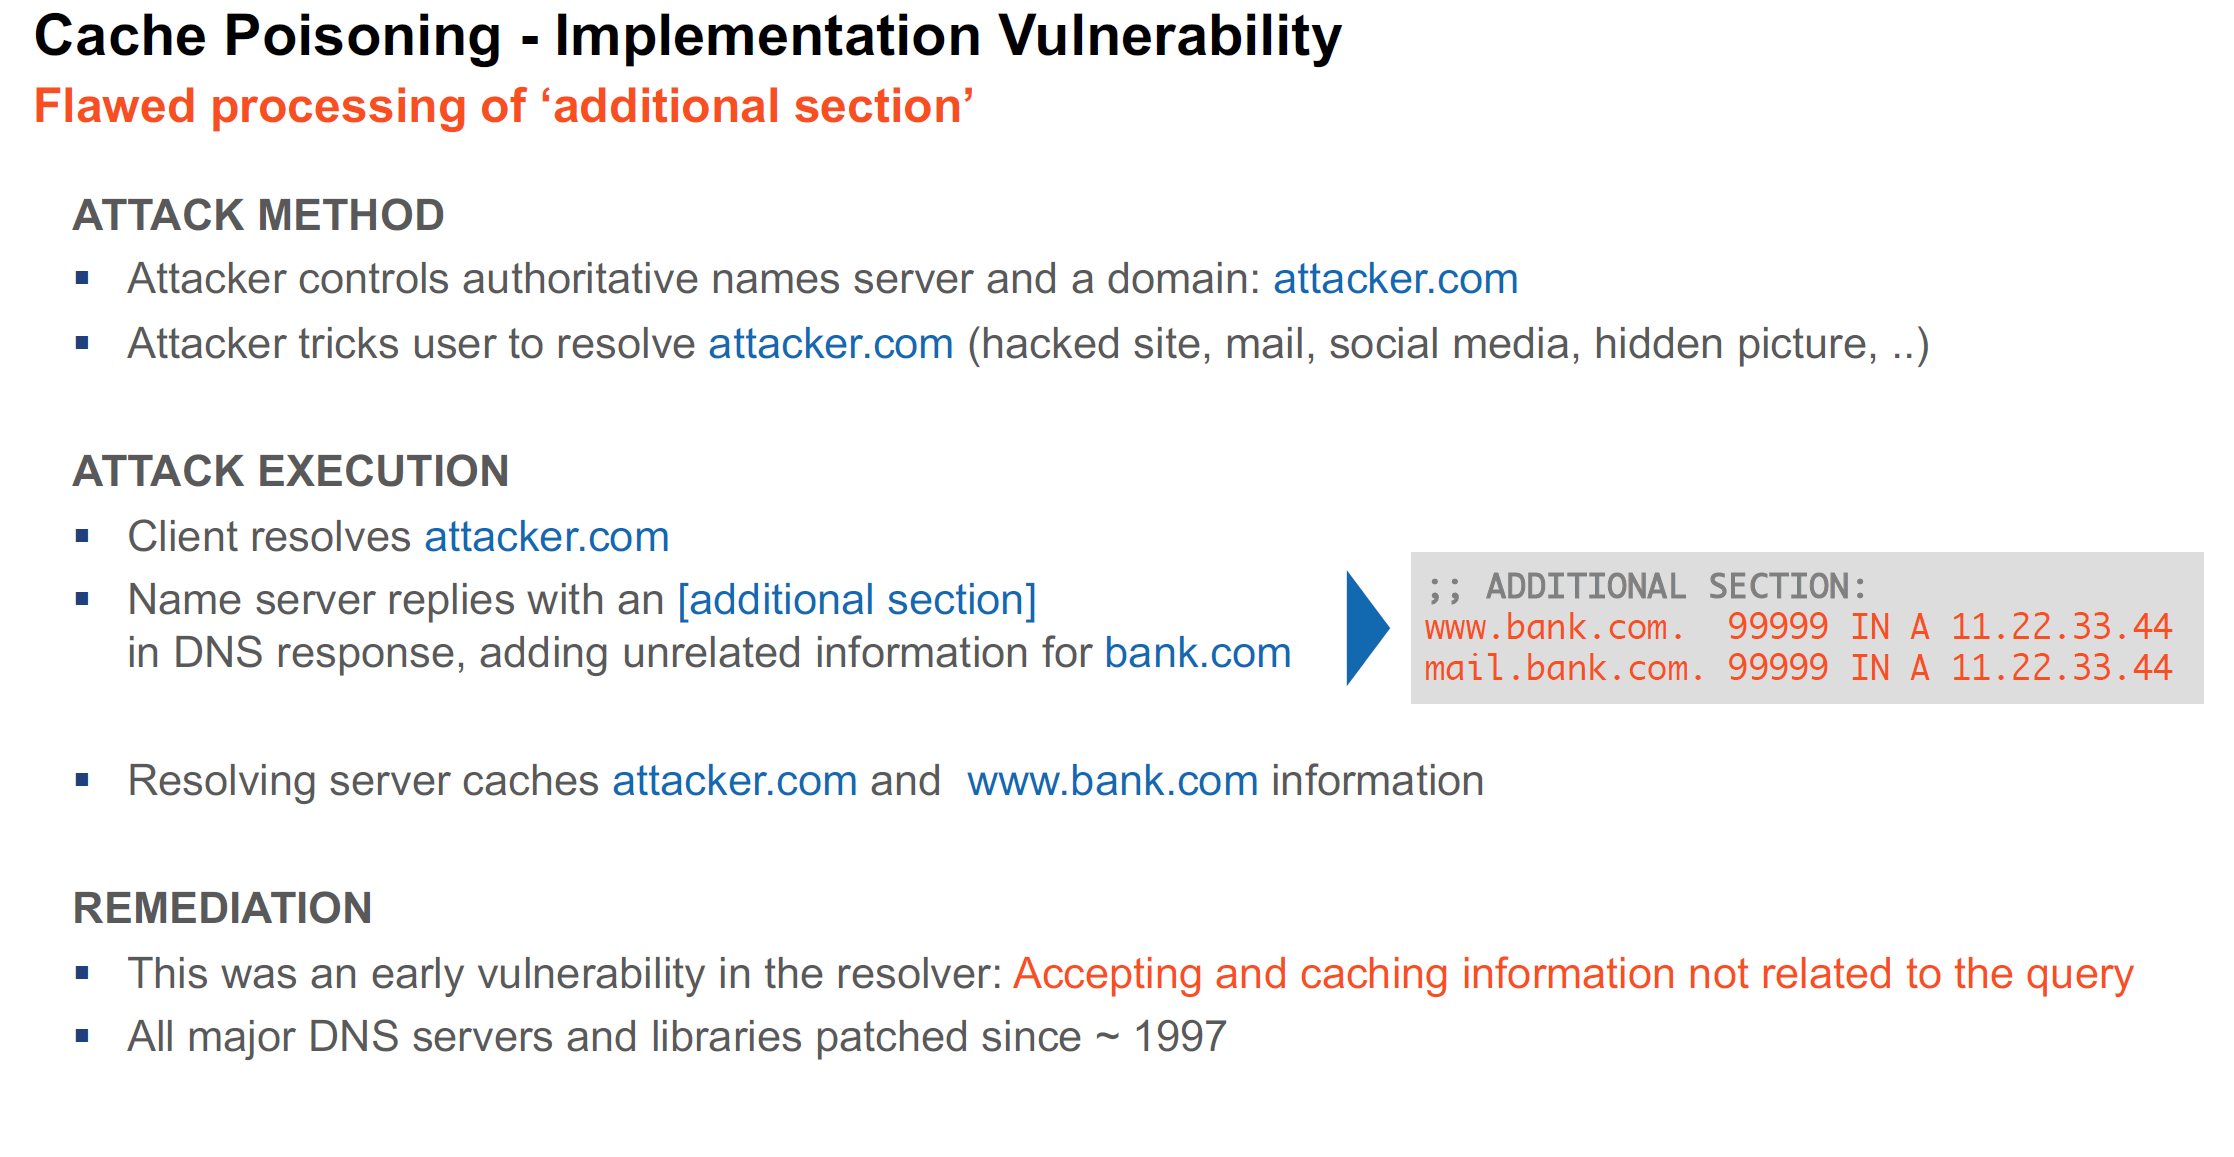
\includegraphics[width=\linewidth]{Figures/DNS_additional_section.PNG} 
\end{minipage}

\paragraph{Cache Poisoning - Guessing Game}
\begin{itemize}
    \item Attacker sends DNS query to a resolver for a nonexisting subdomain of banking.com, then sends forged response(s) as soon as the resolver queries the name server. If the injected response gets accepted the attacker has successfully injected a fake ip address for banking.com. 
    \item Only knowing the txid and source port prevent the attacker to insert his own information.
    \item At best attacker can guess: port and txid entropy (at max): $2^{16} x 2^{16} = 65'536^2$ bad odds!
    However, this is theory and we live in the real world.
    \item Attacker needs to wait until next race if his response is late or wrong - the correct info is cached until TTL expires.
\end{itemize}

\paragraph{Kaminsky Attack:} Use some tricks to make the odds turn: 
\begin{itemize}
    \item Attacker can force a server to look sth up: client-server request \& response round-trip takes time. It takes attacker no time to immediately send face response.
    \item Try lots of random txid and send a reply for each of them simultaneously.
    \item Lookup [1-100].www.bank.com -> attacker gets 100 races
    \item When found correct combination of txid and src port send additional section in reply similar to previous attack.
    \item This attack was mitigated by randomizing src port.
\end{itemize}

\paragraph{SADDNS Attack:}
\begin{itemize}
    \item When a DNS server issues a query, its source port effectively becomes open to the public.
    \item Trigger the DNS server to send a query on target server (src port becomes open to public)
    \item Mute victim Name Server to delay response (buy time for attacker)
    \item Scan port range with UDP to identify open source port.
    \item Once the source port nr is known, the attacker simply injects a large number of spoofed DNS replies bruteforcing the txid.
    \item \textbf{Mitigations:} DNSSEC, Disable ICMP port unreachable to disallow portscanning, Randomize ICMP global rate limit.
\end{itemize}

\paragraph{Learned Lessons}
\begin{itemize}
    \item Source port randomness is not everywhere truly random.
    \item Txid has insufficient randomness and entropy (only 16 bit).
    \item Birthday Paradox: Multiple outstanding requests for the same resource records.
\end{itemize}

\subsection{Compromised Configuration}

\paragraph{Attack Domain Registrar}
Top Level Domains are controlled by specific domain registrars (selected by IANA). Compromise Domain Registrar, Second level domains (SLD) are registered with one of the domain registrars of the TLD.

\begin{itemize}
    \item The DNS information is as secure as the Web App, Registration Processes, or the Passwords of the registrar and the domain owner.
    \item Hack the Web App of the domain registrar, Brute-force users password.
    \item Then change registration entries directly at the registrar. Lock owner out of his account.
\end{itemize}

\paragraph{Attack Network \& Local Configuration:} Insecure provisioning of DNS setting
Manipulate DNS configuration settings on internal network or local host. Have target point to attackers name server.
\begin{itemize}
    \item WAN Network: Scan ISP networks, identify vulnerable routers or weak/default passwords. Attack poorly protected client router of Internet Service Providers (ISP)
    \item LAN Network: Attack client router or DHCP server directly. Attack DHCP exchange in local network (Cache poisoning against DHCP: attacker replies faster than DHCP)
    \item Local Host: Manipulate DNS local hosts settings on compromised machine. Malware changes local DNS configuration (e.g. the file for static mapping of names to IPs \texttt{/etc/hosts} for linux, disable Antivirus updates by changing the mapping from download-site, or mapping of name server). Possible exploits are ad manipulation (Google ads), phishing (credit cards, online banking) or selling software (fake iTunes shops).
\end{itemize}

\paragraph{Name Server Roles}
Recursive name servers that resolve queries for anybody are a security problem:
Can be abused to launch powerful DDoS attacks from anywhere. DNS queries are typically transmitted over UDP - they are fire and forget. The source IP can be spoofed and the receiver has no way of determining its veracity before responding. The attacker will spoof the srcIP to the victim's IP - the response will thus be reflected to the victim and overload his servers. DNS also is capable of generating a much larger response than query (e.g. \texttt{dig ANY isc.org @x.x.x.x} query is 64 bytes, the response is 3,223 bytes). There are many powerful and well connected DNS servers, which can be abused to redirect large DNS responses to any target. The key to this attack are \textit{open} DNS resolvers (recursive resolver that replies to any DNS query, coming from any device
on the Internet).

\begin{itemize}
    \item Authoritative Server: responds to queries from any source. Non recursive queries. Only with data it is authoritative about.
    \item Cache/Recursive Resolver: Respond to local network only. Recursive queries. Should attempt to resolve any legitimate request
\end{itemize}

\textbf{Mitigation:} Source IP verification (reject packets with source addresses not reachable via the actual packet’s path), disable recursion on authoritative name servers, limit recursion to authorized clients, Response Rate Limiting (RRL).\\
However, the main mitigation is hosting a service on different locations in the internet, s.t. it gets harder for an attacker to target all possible locations. Using BGP anycast, the same IP address is advertised on different locations on the internet.\\
A user is directed to the nearest service location. This helps to distribute the load on different sites. There are CDN services like Akamai or CloudFlare that offer this as a service.
\\
On TCP, this attack would not work as is since the second message after the TCP SYN is not the DNS response but the TCP SYN ACK. The TCP ACK would go to the victim (due to the srcIP spoofing). The DNS response would be the second message sent by the server. However, the attacker could reply with the third handshake message + payload after intercepting the replies and dropping them. If the attacker is not Dolev-Yao, which is often the case, the attack would become tricky to perform.

\subsection{Domain Name System Security Extensions (DNSSEC)}

DNSSEC attempts to add security, while maintaining backward compatibility to the
existing DNS. DNSSEC is a set of extensions to DNS to provide resolvers:
\begin{itemize}
    \item origin authentication of DNS data
    \item authenticated denial of existence
    \item integrity
    \item But not availability or confidentiality.
\end{itemize}

\paragraph{DNSSEC Key Features:}
\begin{itemize}
    \item DNSSEC zone data is digitally signed using a private key for that zone. A DNS server receiving DNSSEC signed zone data can verify the origin and integrity of the data by checking the signature using the public key for that zone.
    \item DNSSEC can protect any data published in the DNS
\end{itemize}

\paragraph{Protection Process:} 
\begin{enumerate}
    \item Each DNS zone signs its data using a private key (recommended to do offline).
    \item A query for a particular record returns: The requested resource record set, a signature (SIG) of the requested resource record set.
    \item The resolver authenticates response using public key.
\end{enumerate}

\paragraph{DDNSSEC Resource Records:} List of added RR in dnssec

\begin{minipage}{\linewidth}
    \centering      
    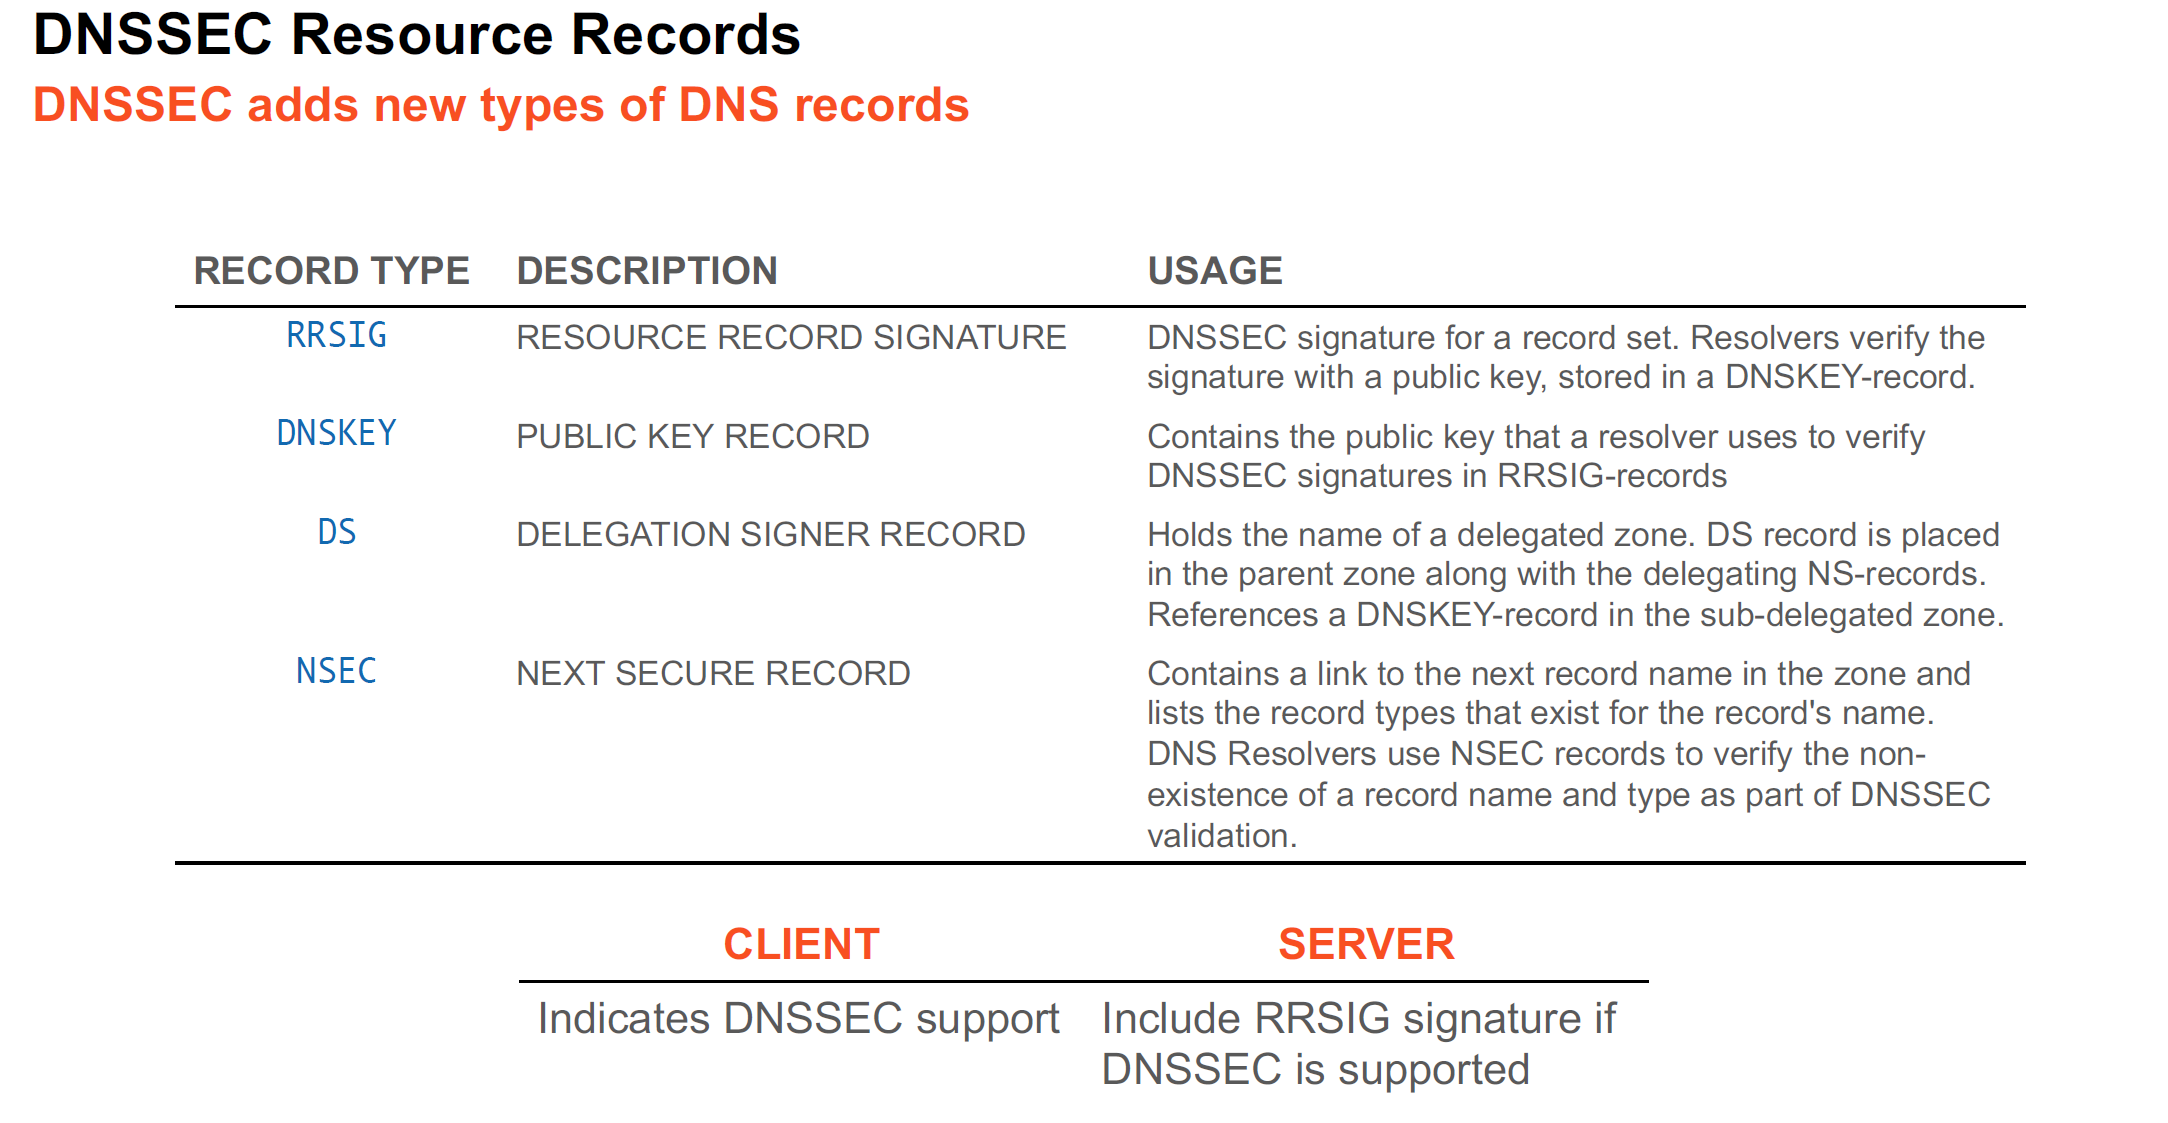
\includegraphics[width=\linewidth]{Figures/DNS_dnssec_rr.PNG} 
\end{minipage}
The DS record contains a hash of the KSK (key signing key) belonging to the
child zone. Once the DNS resolver knows the contents of DS, it can retrieve the KSK and ZSK (zone
signing key) belonging to the child zone. KSK is checked against DS. ZSK is validated using
the KSK. Finally, if the child zone is the actual target of the query, the answer
can be checked by using the ZSK.

\paragraph{DNSSEC Pros and Cons:} Advantages and disadvantages of dnssec
\begin{minipage}{\linewidth}
    \centering      
    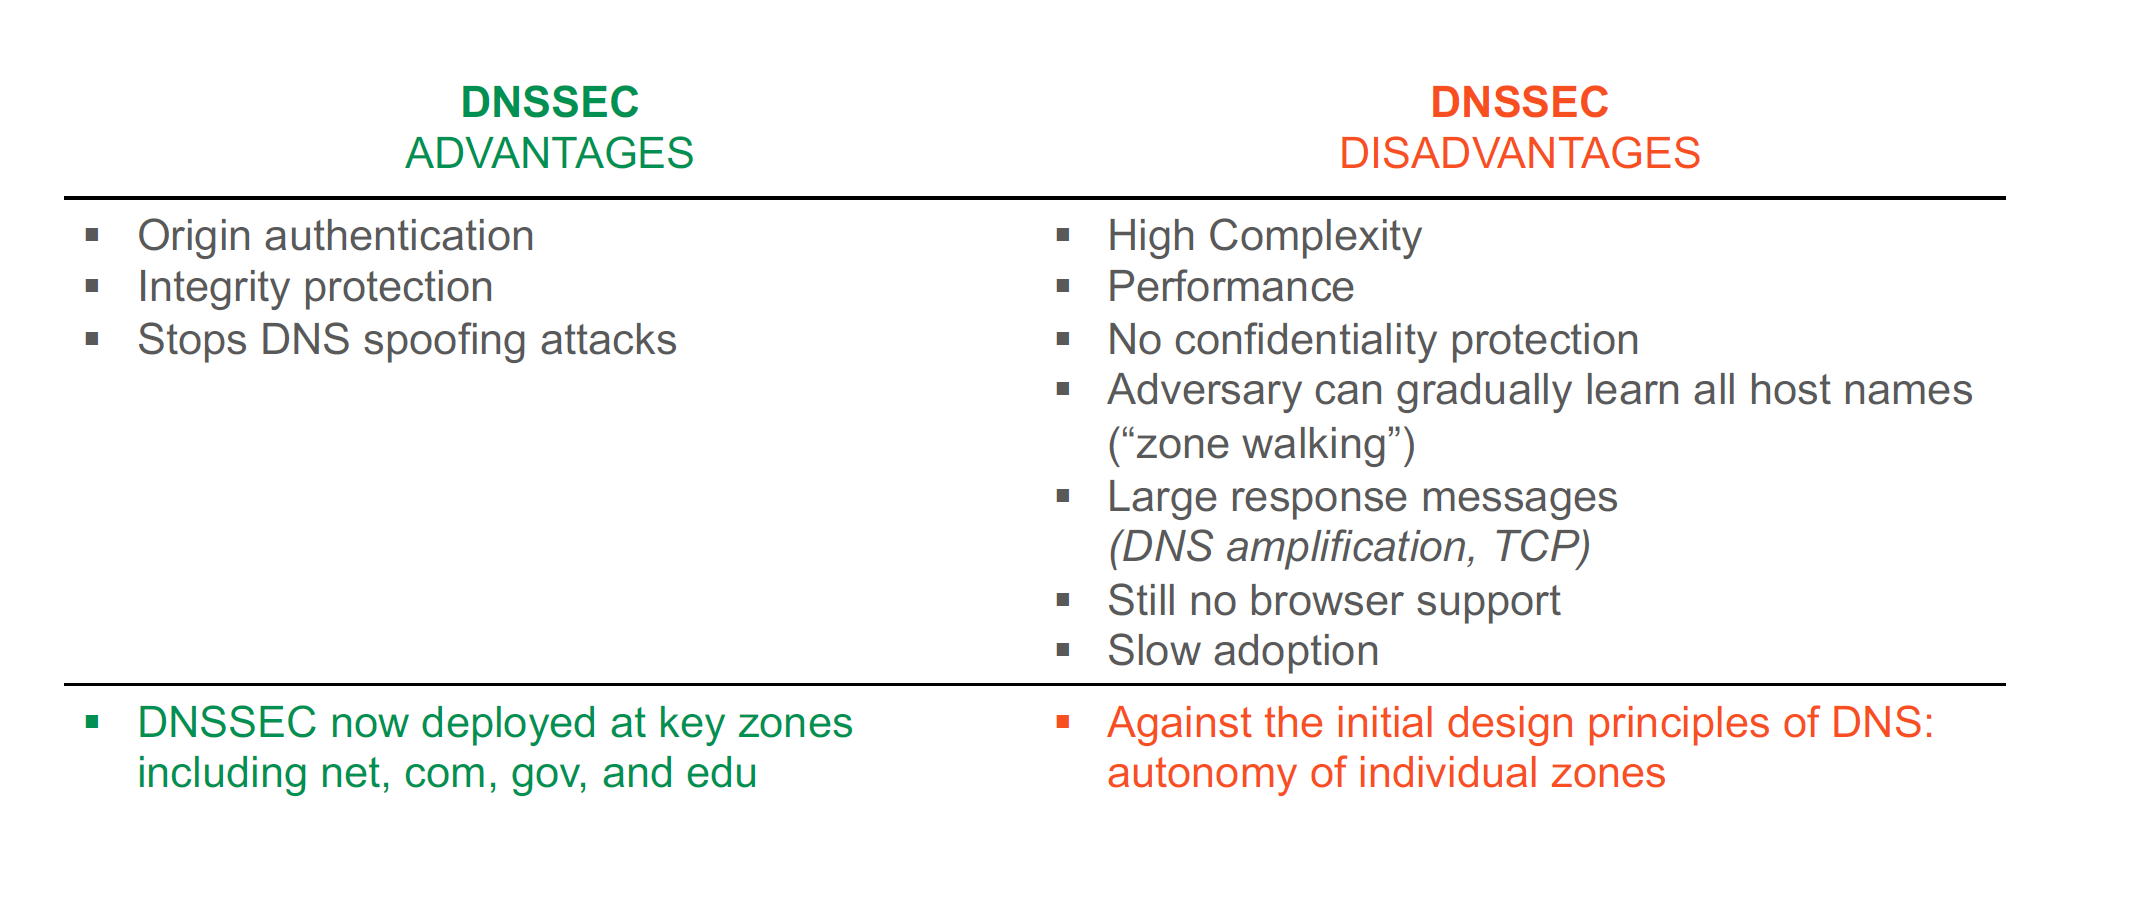
\includegraphics[width=\linewidth]{Figures/DNS_dnssec_advantages.PNG} 
\end{minipage}

\subsection{DNS over HTTPS (DoH) or TLS (DoT)}
DoT users service specific port 853, which might be filtered by firewall/attacker. DoH users standard HTTPS port (443), usually no filtering, easy integration.
Problems:
\begin{itemize}
    \item DNS messages are not protected from eavesdropping (even with DNSSEC)
    \item DNS request are an easy way of tracking users (by the ISP or intelligence services)
\end{itemize}

DOH would solve some attacks on DNS such as DNS spoofing, mass-logging of DNS requests, DNS amplification/reflection, cache poisoning, etc. However, there are disadvantages. With DOH, local caches are no longer possible – each query needs to reach the remote DoH resolver. In the case of large providers, load and latency are not a problem: anycast is used to respond to the queries in a geographically distributed way. However, this concentrates even more power in the hands of a few companies (Google, Cloudflare, etc.); the internet gets even more centralized.



